The results visualization system provides a graphical summary of the progression of an optimziation. It was written using Ruby On Rails and takes advantage of two graphical plotting tools: gcharts and graphviz. Gcharts is used to generate the graphcial plots of relevant optimization metrics from different optimizations. The graphviz package is used to render images of the 

\subsection{Optimization Metrics}

\subsection{TM Representation}
The vizualization of individual TMs provides a valuable tool for their inspection. There are litterally thousands of TMs created over the course of an optimziation, and graphviz package allows or the creation of a state transition diagram for quick visual inspection of particular TMs. Figure \ref{fig:example_TM} is the state transition diagram for the example TM in Table \ref{tab:example_TM}. This visual representation is much easier to interperate than the state transition table. 

\begin{figure}[!hbp]
	\centering 
	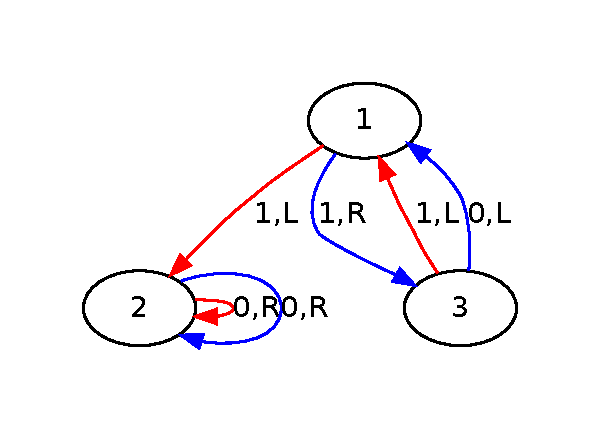
\includegraphics[width=.8\textwidth]{images/example_TM}
	\caption{State transition diagram for notional 3-state TM. Edge color indicates the bit being read from the tape (red=0,blue=1). Edge label indicates the write bit and movement direction for a given transition.}
	\label{fig:example_TM}
\end{figure}

